%
% Firewall
%
% Aleph Objects Firewall
%
% Copyright (C) 2014, 2015, 2016 Aleph Objects, Inc.
%
% This document is licensed under the Creative Commons Attribution 4.0
% International Public License (CC BY-SA 4.0) by Aleph Objects, Inc.
%

\section{Overview}
Aleph Objects has recently deployed pfSense firewalls, replacing OpenBSD.
Most servers and workstations run GNU/Linux, which uses iptables.


\section{iptables}
iptables is part of the Netfilter project and has been included by default in
the Linux kernel for many years.

\begin{figure}[h!]
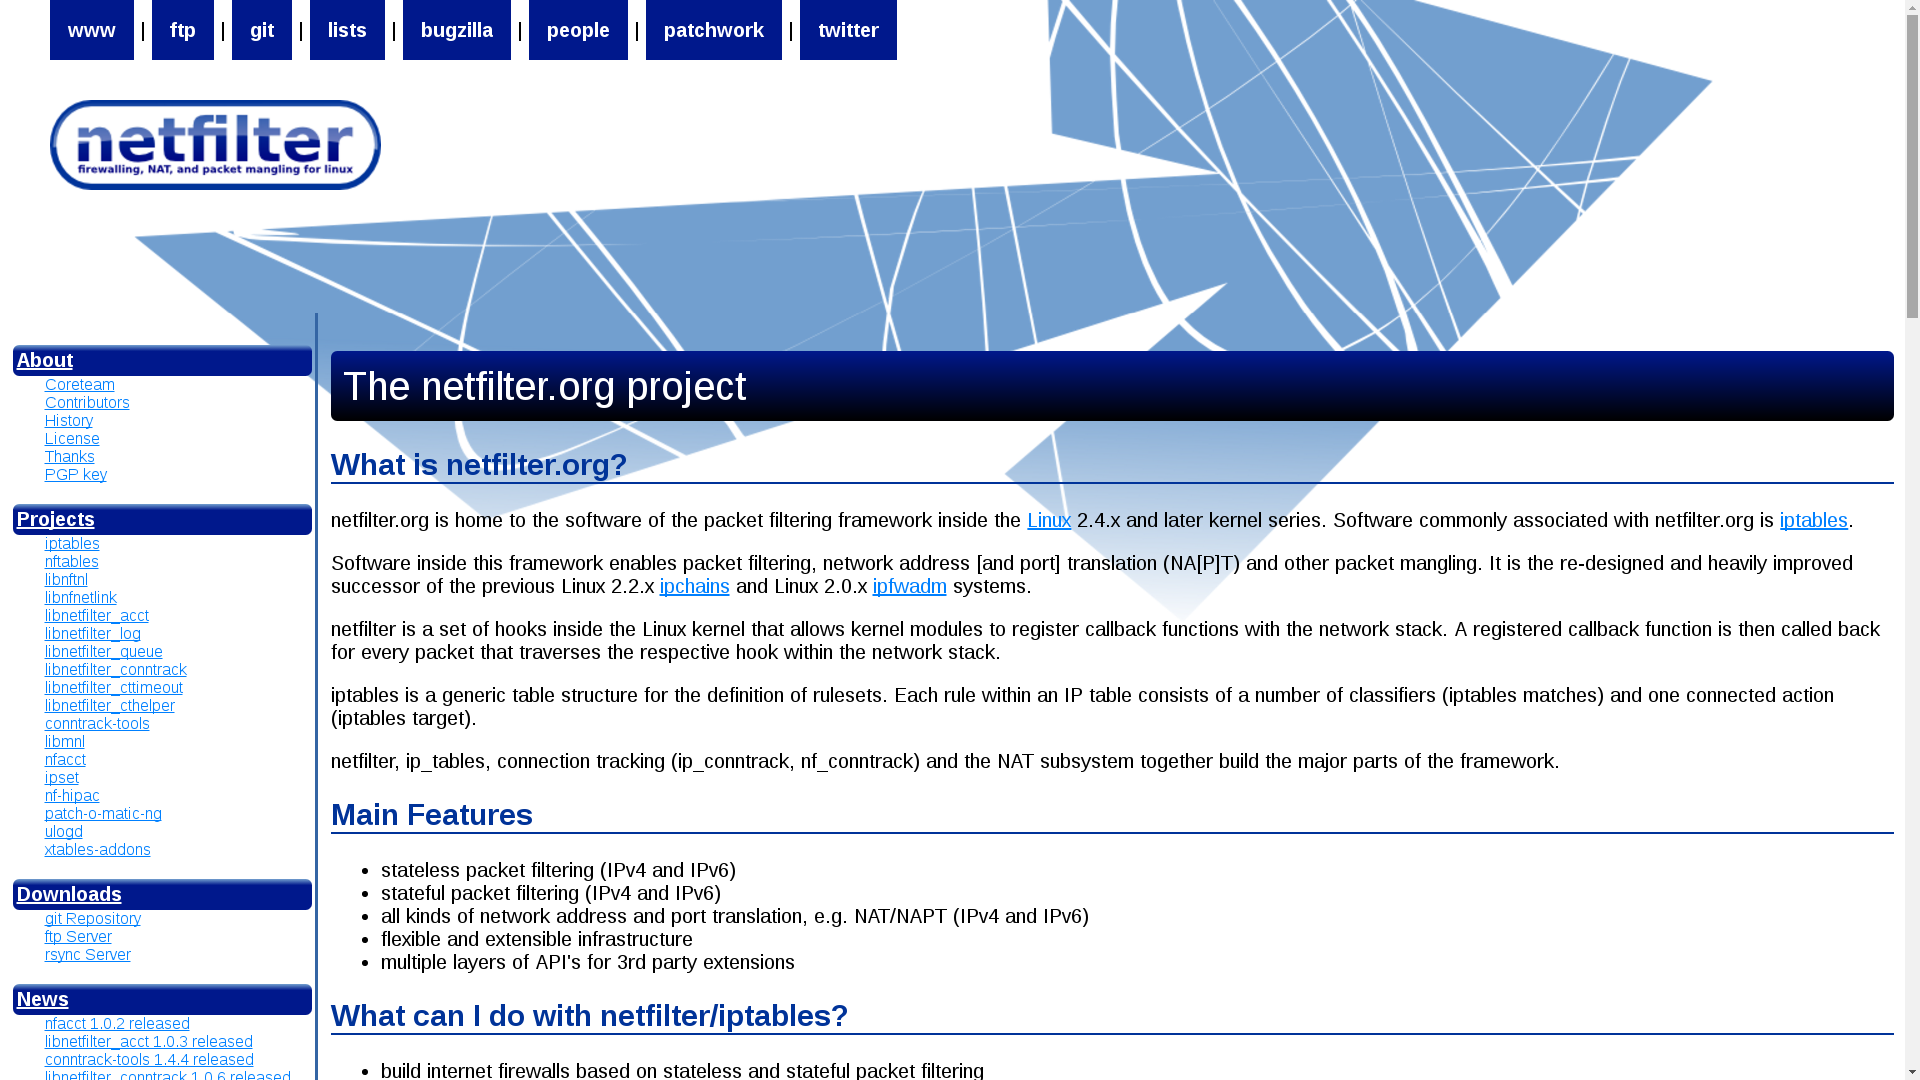
\includegraphics[keepaspectratio=true,height=1.10\textheight,width=1.00\textwidth,angle=0]{www-netfilter.png}
 \caption{Netfilter Website}
 \label{fig:www-netfilter}
\end{figure}


\section{pfSense}
\href{https://www.pfsense.org/}{pfSense} --- ``Free, open source customized
distribution of FreeBSD specifically tailored for use as a firewall and router
that is entirely managed via web interface.''

pfSense was selected as Aleph Objects core router/firewall for backbone
connections.

\begin{figure}[h!]
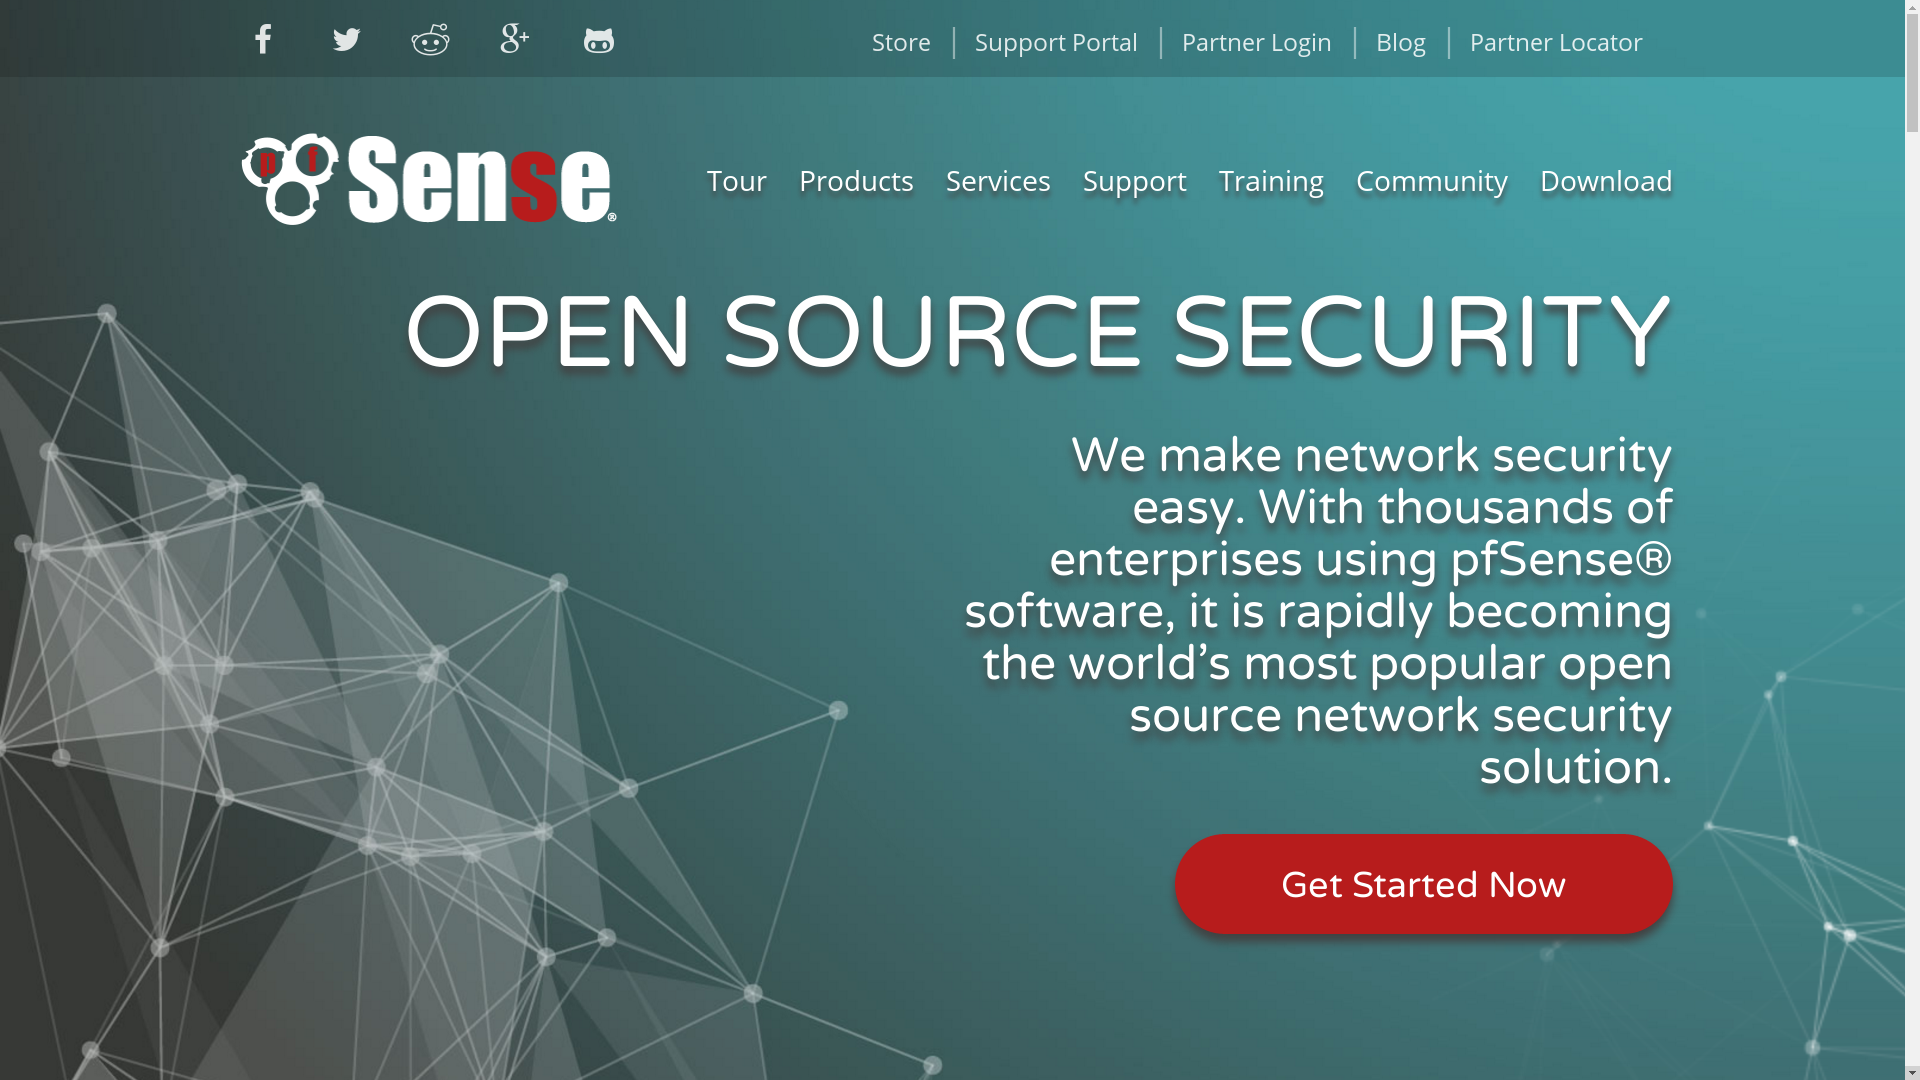
\includegraphics[keepaspectratio=true,height=1.10\textheight,width=1.00\textwidth,angle=0]{www-pfsense.png}
 \caption{pfSense Website}
 \label{fig:www-pfsense}
\end{figure}

\subsection{Configuration}
\begin{enumerate}
 \item Connect via USB cable. 115200 baud, 8N1, no flow control.
 \item Copy MAC address to main DHCP/DNS server, and reserve IP address.
 \item Set IP for LAN (e.g. 192.168.1.1)
 \item Set IP for WAN, disable IPv6
 \item Log in to firewall (e.g. https://192.168.1.1).
       Initial pass admin/pfsense.
 \item Start Wizard, hit Next.
 \item pfSense Gold, Next.
 \item Hostname: set hostname.
 \item Set WAN, LAN, password, etc.
 \item Hit Reload, and the wizard is done.
 \item System --> User Manager. Click Add. Add Username, Password, Full name, Experation date leave blank. Move to add to Group membership ``admins'' (presuming this is an admin). Add ssh key, if you want to ssh in. Certificate, leave blank for now (can be used for OpenVPN/RADIUS). 
 \item Log out and log back in as newly created user.
 \item Goto System --> Advanced. Under Admin Access. Set TCP port to randomish port between 1 and 65535. This will be the new pfSense web interface port address. Max processes: 16(2 is too low, not sure what is ideal). Check WebGUI redirect to disable port 80. Check enable Secure Shell Server. Disable password login. Pick randomish port for SSH. Check to password protect Console menu. Save.
 \item At this point, you can optionally SSH into the firewall if a key was set up for the user.
 \item Under System --> Advanced, Networking. Uncheck Allow IPv6, to disable IPv6 (yay!). Check boxes for: Hardware Checksum Offloading, Hardware TCP Segmentation Offloading, Hardware Large Receive Offloading. These need to be disabled because/if Suricata is used in Inline mode. If it isn't, these can be unchecked and if the hardware is good/can handle it, it will likely be faster. (Side note, enabling Hardware Checksum Offloading breaks networking in a KVM.) Save.
 \item System --> Advanced, Miscellaneous. Cryptographic Hardware should be set to AES-NI for any hardware from pfSense. For other hardware, check dmesg. Thermal Sensors: Intel Core* CPU on-die thermal sensor. Hard disk standby time, 6 minutes (not sure this really has any effect). Host UUID, check Do NOT send HOST UUID with user agent. Save.
 \item System --> Notifications. Check for Disable Growl Notifications and Disable SMTP. Save.
 \item System --> Cert. Manager. Under CAs, click Add. Method: Import an existing Certificate Authority. Descriptive Name: ``GandiStandardSSLCA2''. Get the cert from \url{https://www.gandi.net/static/CAs/GandiStandardSSLCA2.pem} and paste into Certificate data. Certificate Private Key, blank. Save.
 \item System --> Cert. Manager. Under Certificates, click Add. Method: Create a Certificate Signing Request. Descriptive Name, use the hostname of the firewall being setup. Key length 4096, Digest Algorithm sha512. Country Code US, etc. Common name, use hostname of firewall. Save.
 \item System --> Cert. Manager, Under Certificates, the new cert added above, click Export Request mini-icon. Gandi: Standard SSL, single address, 3 year. Paste in the CSR exported from the mini-icon into Gandi. Select Apache/ModSSL for Software used in Gandi, and if it says the correct ``Main domain (CN)'', hit Submit in Gandi. Delete any .req file that was downloaded by browser. Gandi: Validation by email (probably). It will take ~10+ minutes to get verification back from Gandi (not instant).
 \item System --> Cert. Manager, also import any of our own CAs and Certificate Revocations, if any.
 \item System --> General Setup. Check all looks good. Top Navigation: Fixed (Remains visible at top of page). Hostname in Menu: Hostname only. (DNS servers can be bound to particular interfaces here, if needed in multi-WAN). Save.
 \item Firewall --> Rules. LAN interface, click the pencil to edit the IPv6 line. Change Action to Reject. Change Source to any. Change Description to ``Default Reject LAN IPv6''. Save. Apply Changes.
 \item Firewall --> Rules. Under LAN interface, click the Copy mini-icon to copy the IPv6 line. Change Action to Block. Interface to WAN. Change Description to ``Default Block WAN IPv6''. Save. Apply Changes.
 \item Services --> DNS Resolver. Enable (default). Network Interfaces: just select LAN and localhost. Outgoing Network Interfaces: WAN, LAN, localhost. Add checks for DHCP Registration, Static DHCP. Save. Apply Changes.
 \item Services --> DNS Resolver, Advanced Settings. Add checks for: Prefetch Support, Prefetch DNS Key Support. Increase Messge Cache Size to 50 MB or so (?).Save. Apply Changes.
% \item Services, Dynamic DNS. Setup.
 \item Status --> System Logs
 \item When WAN is first connected, do System --> Update.
\end{enumerate}


\subsection{NAT}
Network Address Translation.

\begin{itemize}
 \item VoIP using SIP is often a problem behind a NAT.
 \item Enable Keepalives in Grandstream phones to connect to the Asterisk server.
 \item Disable ALG (Application Level Gateway) in any consumer/home routers.
\end{itemize}


\subsection{Traffic Shaping}
\begin{itemize}
 \item Prioritize admin ssh to firewalls/servers (in case of DoS, etc.)
 \item Prioritize VoIP
 \item De-prioritize SMTP, etc...
\end{itemize}

\subsection{pfBlockerNG}
\begin{itemize}
 \item IP blocklists for botnets, etc.
\end{itemize}


\subsection{Suricata}
Suricata is being used as an Intrusion Detection System.
It is preferred over Snort as Suricata is multithreaded and Snort isn't.

\begin{figure}[h!]
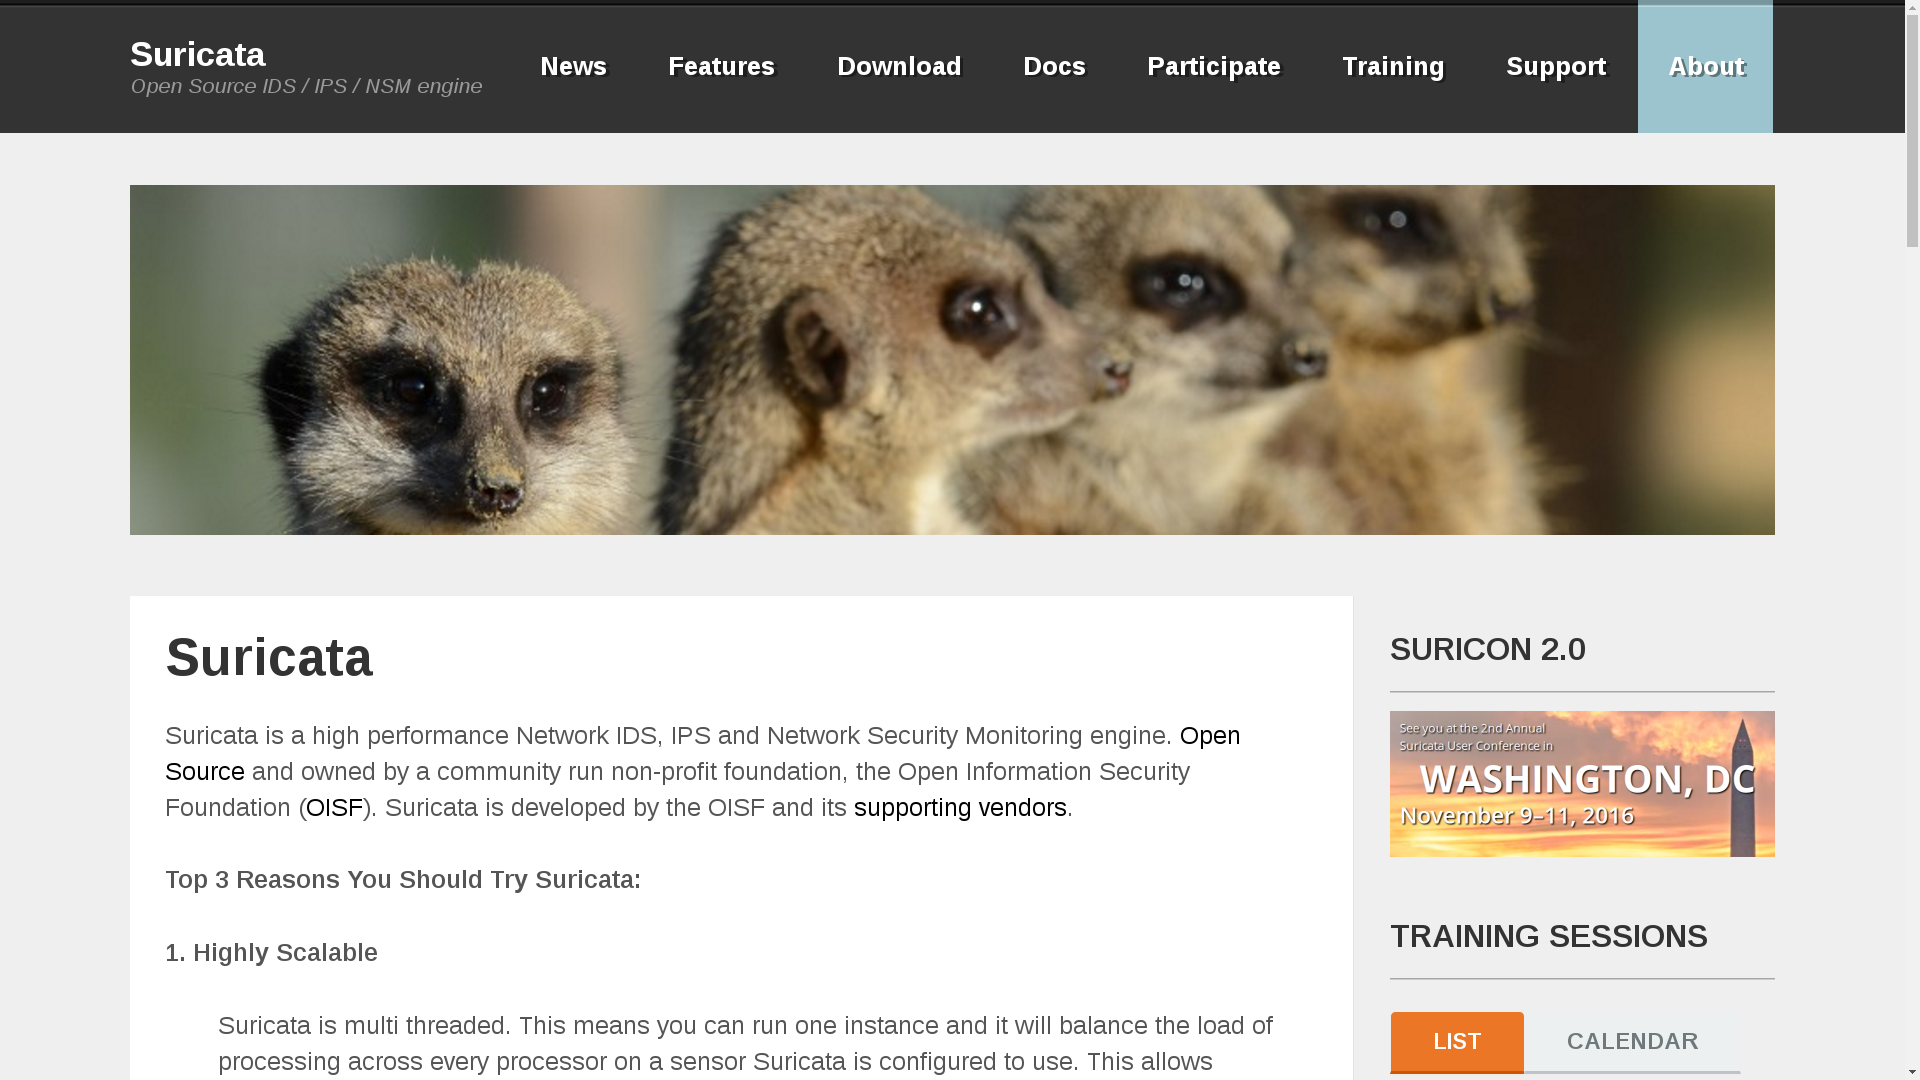
\includegraphics[keepaspectratio=true,height=1.10\textheight,width=1.00\textwidth,angle=0]{www-suricata.png}
 \caption{Suricata Website}
 \label{fig:www-suricata}
\end{figure}

\begin{itemize}
 \item barnyard2
 \item Snort Blacklists
 \item Emerging Threats Blacklists
 \item GeoIP
 \item Alerts, Blocks, Suppress
 \item SID
\end{itemize}


\subsection{DHCP}
For DHCP services, pfSense uses Dnsmasq, which is also used for DNS
forwarding.

\begin{itemize}
 \item Disable IPv6.
 \item tftp netboot installs.
 \item Static mappings.
\end{itemize}


\subsection{NTP}


\subsection{OpenVPN}
\begin{figure}[h!]
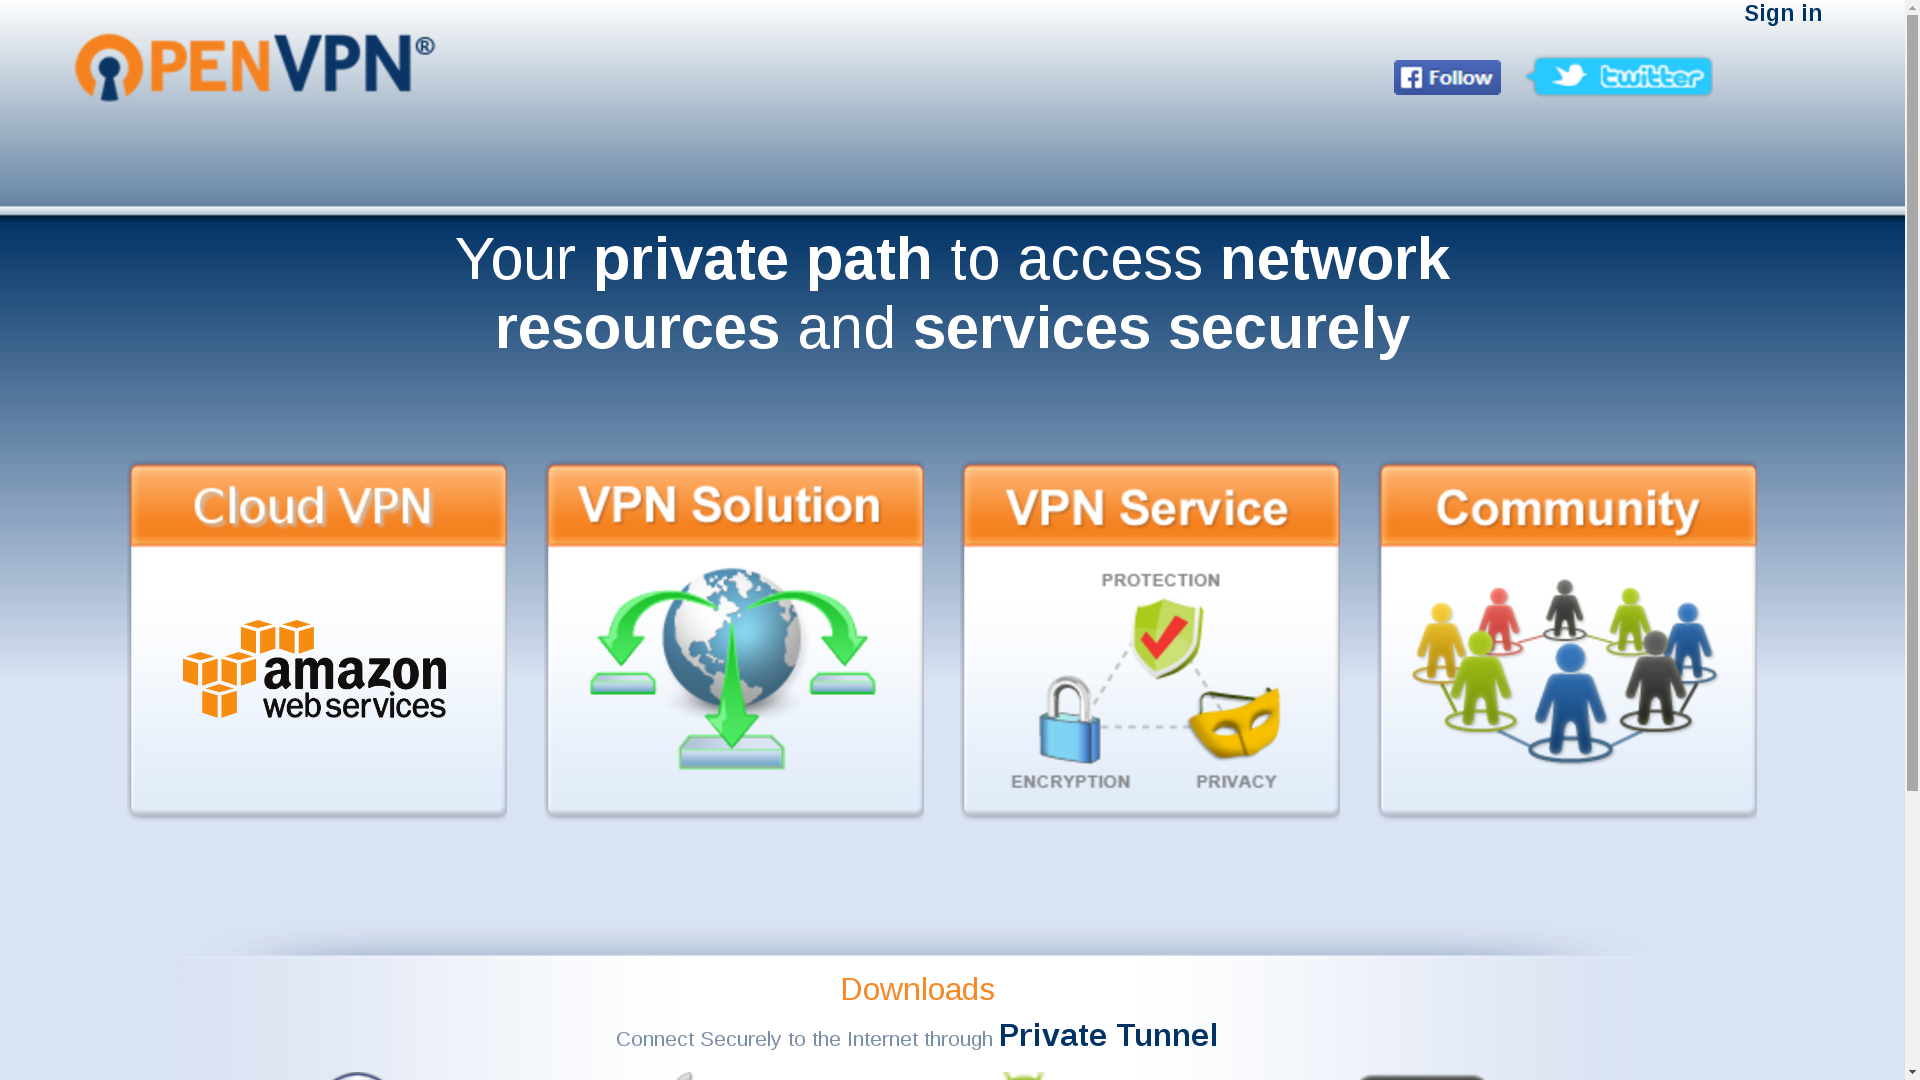
\includegraphics[keepaspectratio=true,height=1.10\textheight,width=1.00\textwidth,angle=0]{www-openvpn.png}
 \caption{OpenVPN Website}
 \label{fig:www-openvpn}
\end{figure}


Virtual Private Networks.


\href{https://www.openvpn.net/}{OpenVPN} --- ``OpenVPN is a full-featured open source SSL VPN solution that accommodates a wide range of configurations, including remote access, site-to-site VPNs, Wi-Fi security, and enterprise-scale remote access solutions with load balancing, failover, and fine-grained access-controls.''

\begin{itemize}
 \item Network design (e.g. many point to point, one central server, etc.).
 \item Main OpenVPN server.
 \item Other internal servers.
 \item External servers private connections.
 \item Laptops.
 \item Mobiles.
 \item SSL certificates.
 \item AES-256-CBC is hardware accelerated on pfSense routers.
 \item SHA512 Auth digest algorithm
 \item Hardware Crypto: BSD cryptodev engine
\end{itemize}


pfSense ships with pre-generated DH keys, due to ``heavy computation''.
This can take an hour for 4096.
\begin{minted}[frame=single]{sh}
/usr/bin/openssl dhparam 1024 > /etc/dh-parameters.1024
/usr/bin/openssl dhparam 2048 > /etc/dh-parameters.2048
/usr/bin/openssl dhparam 4096 > /etc/dh-parameters.4096
\end{minted}



\subsection{Captive Portal}
The Captive Portal for Aleph Mountain building wifi services.


\subsection{SSL Certificates}
pfSense makes it very easy to generate Certificate Signing Requests (CSRs),
which can be send to Gandi.net to get issued a ``properly'' signed SSL
certificate.


\subsection{ssh}
OpenSSH from OpenBSD is used. The BSD shell is a bit different from GNU.


\subsection{DNS}
DNS forwarding is provided by Dnsmasq.

\begin{figure}[h!]
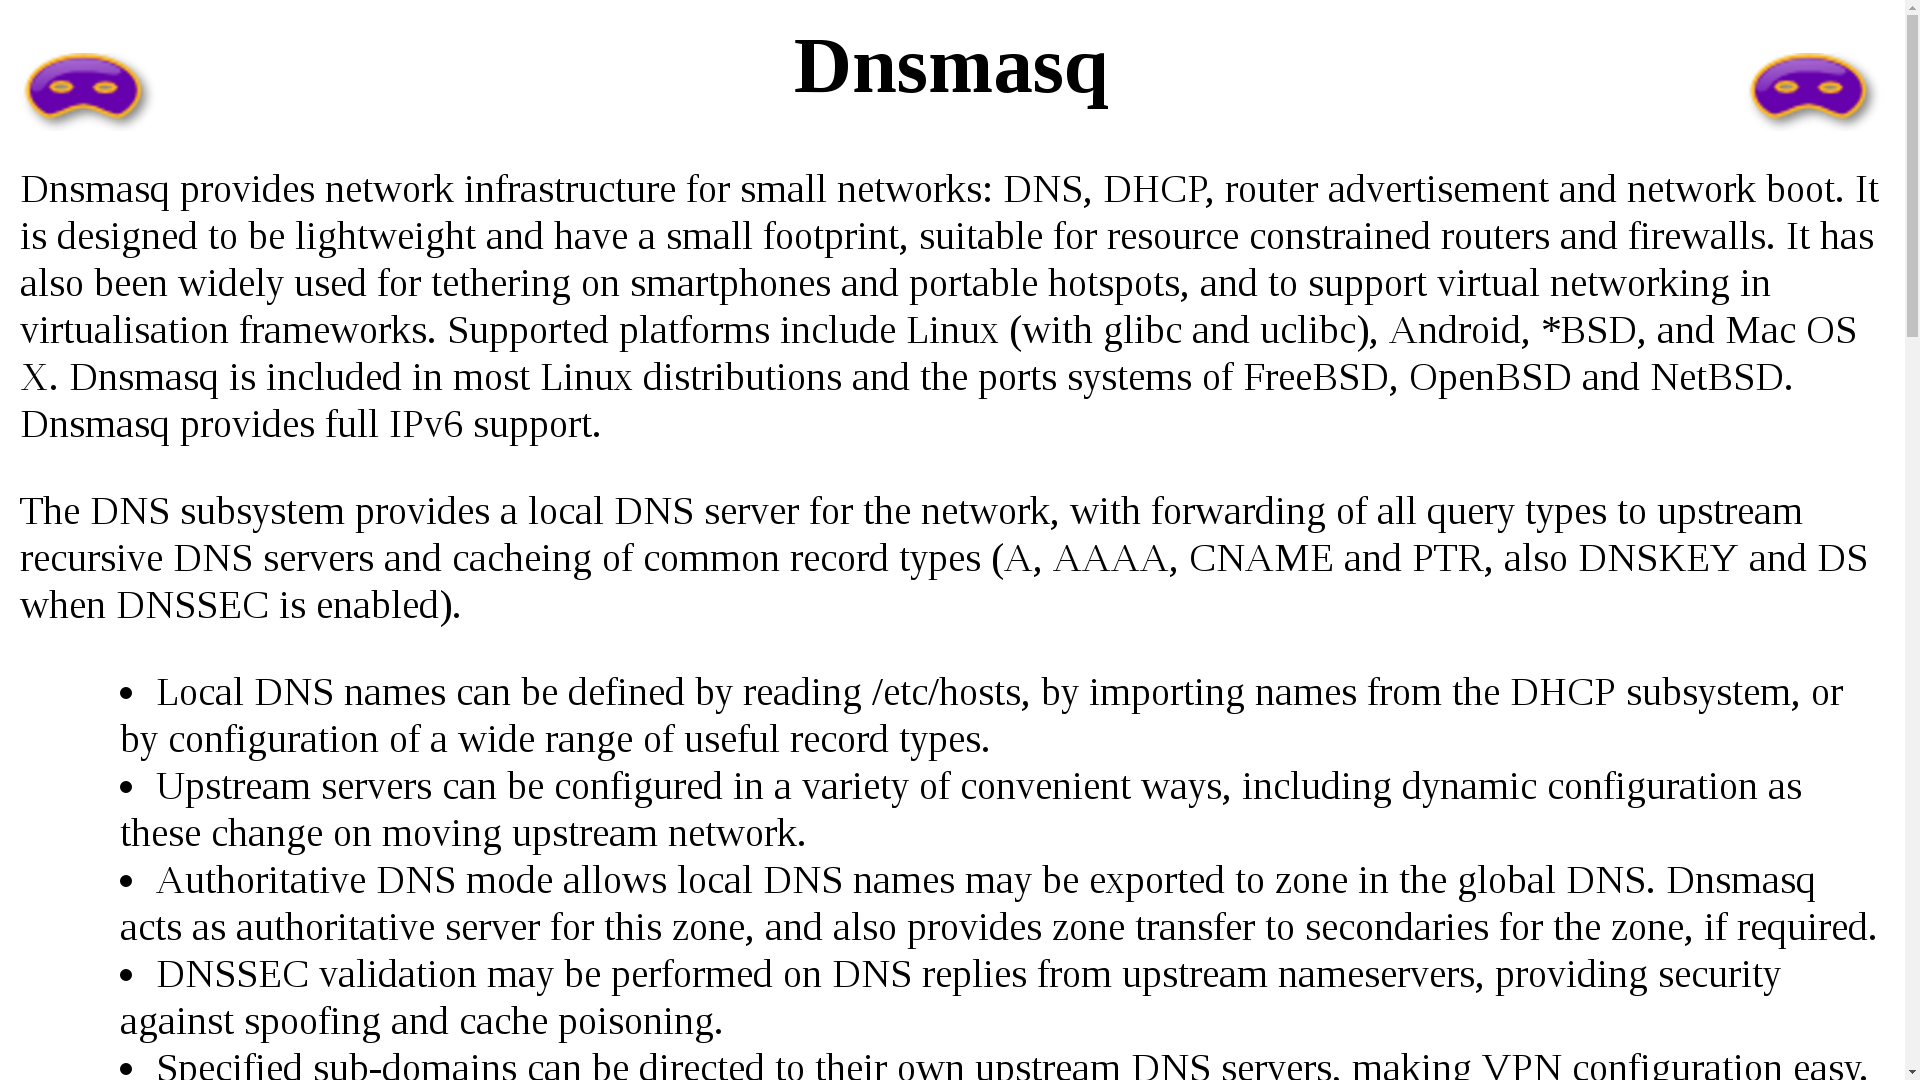
\includegraphics[keepaspectratio=true,height=1.10\textheight,width=1.00\textwidth,angle=0]{www-dnsmasq.png}
 \caption{Dnsmasq Website}
 \label{fig:www-dnsmasq}
\end{figure}



\subsection{Routing}
\begin{itemize}
 \item No BGP, OSPF, etc.
 \item Static backbone routes.
 \item WAN failover
\end{itemize}


\subsection{Interfaces}

\begin{itemize}
 \item Gigabit ethernet.
 \item SFP+.
 \item Hardware offloading (e.g. checksums).
\end{itemize}


\subsection{CARP and Synchronization}
CARP can be used to have transparent failover to another firewall, if one
firewall on the network should drop.

Synchronization between CARP firewalls allows easy configuration updates. For
instance, if a configuration change is made to the DHCP server, it can
``instantly'' push to the backup firewall.


\subsection{Reporting}

\begin{figure}[h!]
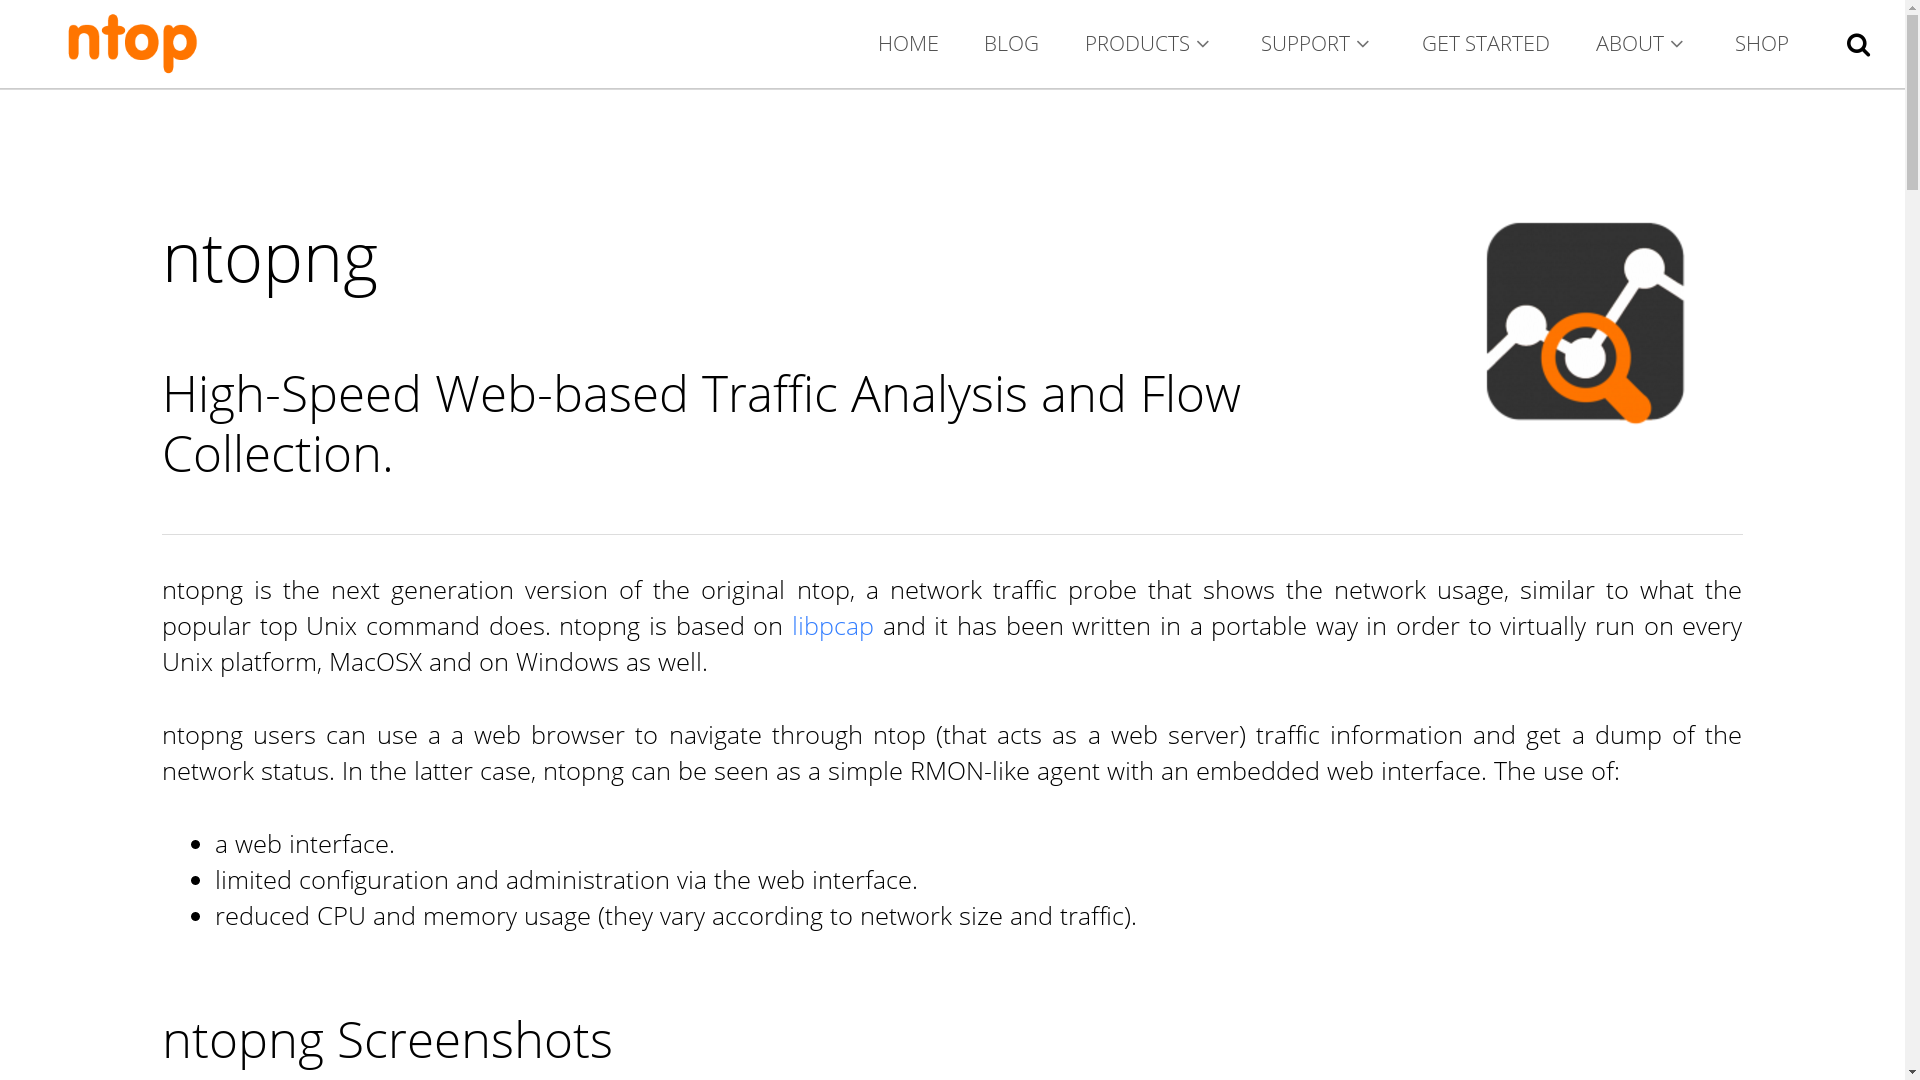
\includegraphics[keepaspectratio=true,height=1.10\textheight,width=1.00\textwidth,angle=0]{www-ntopng.png}
 \caption{ntopng Website}
 \label{fig:www-ntopng}
\end{figure}

\begin{itemize}
 \item Dashboard.
 \item Darkstat.
 \item ntopng (``Network Top Next Generation'' ?).
 \item S.M.A.R.T.
 \item System Temperatures.
 \item MRTG
 \item RRD
\end{itemize}


\subsection{Test Evaluation Install notes}

A few notes from the initial test install:

\begin{itemize}
 \item Released May 18th, 2016.
 \item pfSense-CE-memstick-2.3.1-RELEASE-amd64.img
 \item FreeBSD 10.3 based.
 \item Installer feels like a step back in computing history.
 \item First boot goes to console with lots of useful options.
 \item Web admin wizard mentions pfSense Gold Subscriptions. It doesn't appear to be for non-free software (e.g. isn't baitware).
 \item They sell very nice looking hardware with pfsense pre-installed. With failover systems (CARP).
 \item Load balancing, failover.
 \item Clean and very responsive web interface (based on Bootstrap).
 \item Web based updater to new minor version.
 \item x86 architecture only.
 \item Looks to have good security errata process, following FreeBSD.
 \item Snort threat lists are available. Paid for more recent ones, same as on other snort platforms.
 \item Installation of additional packages is clean, and doesn't appear to offer any non-free.
 \item ClamAV ...
\end{itemize}

